\documentclass[letterpaper,12pt,fleqn]{article}
\usepackage[margin=1in]{geometry}
\usepackage{libertine}
\usepackage{parskip}
\usepackage{enumitem}
\usepackage{amsfonts}
\usepackage{amssymb}
\usepackage{amsthm}
\usepackage{mathtools}
\usepackage{mathrsfs}
\usepackage{siunitx}
\usepackage{tikz}
\usepackage{pgfplots}
\pgfplotsset{compat=1.16}
\DeclarePairedDelimiter{\abs}{\lvert}{\rvert}
\pagestyle{plain}

\begin{document}   

\begin{center}
  \large
  \textbf{Spring 2020 Math 30 Makeup Final Exam}
\end{center}

\vspace{0.5in}

Name: \rule{4in}{1pt}

\vspace{0.5in}

\begin{enumerate}[left=0in]
\item Determine the limits:

  \vspace{0.5in}

  \begin{enumerate}
  \item \(\displaystyle\lim_{x\to0^+}\frac{\abs{x}}{\sin x}\)

    \vspace{1in}

  \item \(\displaystyle \lim_{x\to\infty}\frac{x\arctan x}{1-2x}\)

    \vspace{1in}

  \item \(\displaystyle \lim_{x\to0}\frac{x^3+2}{xe^{x^2}}\)
  \end{enumerate}

  \newpage

\item Using the limit definition of the derivative, find \(f'(x)\) where:
  \[f(x)=\frac{x}{2x+3}\]
  Show your work and \emph{do NOT use differentiation rules}.

  \newpage

\item You are designing sealed plexiglass tanks to be used as part of a biology experiment.  The tanks are
  rectangular in shape and have a square base.  The tanks must have a volume of \SI{1000}{cm^3}.  The material
  that will be used to make the base (bottom) costs \SI{5}{cents/cm^2}.  The material that will be used to make
  the lid costs \SI{4}{cents/cm^2}.  The material that will be used to make the walls costs \SI{10}{cents/cm^2}.

  \bigskip

  \begin{enumerate}
  \item Determine the dimensions of the tank that minimize the material costs.  Round you answers to the nearest
    tenth of a centimeter.

    \vspace{2.5in}

  \item What is the minimum cost, rounded to the nearest cent?

    \vspace{1.5in}

  \item Justify that your answer is indeed the minimum cost.
  \end{enumerate}

  \newpage

\item Let \(f(x)=\ln(x\ln(1+x^2))\).  Find \(f'(x))\).

  \newpage

\item Show all necessary steps:

  \bigskip

  \begin{enumerate}
  \item Differentiate:
    \[g(x)=\cos(\arctan(\sqrt{x})\]

    \vspace{3in}

  \item Find the most general antiderivative of the function:
    \[f(x)=\frac{x^22^x+6}{x^2}\]
  \end{enumerate}

  \newpage

\item A test missile passes over a monitoring station at an altitude of \SI{5}{mi}.  The missile is traveling at
  \SI{520}{mph}.  You are standing at a position that is \SI{12}{mi} from the monitoring station.  At what rate is
  the distance from the monitoring station to the missile changing when the missile passes over you?

  \newpage

\item Find the tangent line to the function:
  \[f(x)=\ln(\cos x)\]
  at \(x=-\frac{\pi}{4}\).

  \newpage

\item Let \(y=x\ln(1+x^2)\):

  \bigskip

  \begin{enumerate}
  \item Find \(y'\).

    \vspace{3in}

  \item Find \(y''\).
  \end{enumerate}

  \newpage

\item Let \(y+2x\cos(y^2-x)=1\).  Find \(\frac{dy}{dx}\) at the point \((1,-1)\).

  \newpage

\item The number of cases of influenza in New York City from the beginning of 1960 to the beginning of 1964 is
  modeled by the function:
  \[N(t)=5.3e^{(0.093t^2-0.87t)}\qquad0\le t\le4\]
  where \(N(t)\) gives the number of cases (in thousands) and \(t\) is measured in years, with \(t=0\) corresponding
  to the beginning of 1960.

  \bigskip

  \begin{enumerate}
  \item Find \(N(0)\) and \(N(4)\).  Explain what these values indicate about the disease in New York City.

    \vspace{3in}

  \item Find \(N'(0)\) and \(N'(3)\).  Explain what these values indicate about the disease in New York City.
  \end{enumerate}

  \newpage

\item Suppose that \(f(x)\) has the graph shown below.  Sketch the graph of \(f'(x)\).  Make sure that you clearly
  show any critical point(s) or asymptote(s).

  \vspace{0.25in}

  \begin{center}
    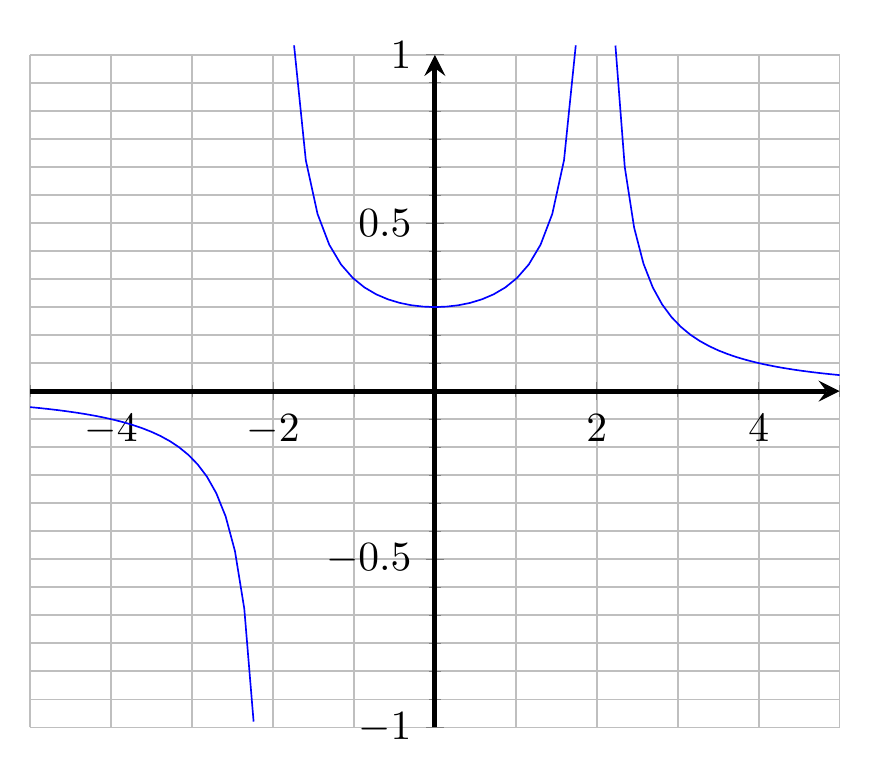
\begin{tikzpicture}[scale=1.5]
      \begin{axis}[
          xmin=-5,
          xmax=5,
          ymin=-1,
          ymax=1,
          axis lines=middle,
          grid=both,
          minor x tick num=1,
          minor y tick num=5,
          axis line style={very thick},
          clip=false
        ]
        \addplot [domain=-5:-2.24,blue] {-1/((x-2)*(x+2))};
        \addplot [domain=-1.74:1.74,blue] {-1/((x-2)*(x+2))};
        \addplot [domain=2.23:5,blue] {1/((x+2)*(x-2))};
      \end{axis}
    \end{tikzpicture}
  \end{center}

  \newpage

\item Is it possible to sketch a graph that satisfies ALL of the following conditions?  If yes then sketch the graph of
  \(f\) below.  Otherwise, explain (in one or two sentences) why not.
  \begin{itemize}
  \item \(f(0)=0\)
  \item \(\displaystyle\lim_{x\to-2^-}f(x)=4\) and \(\displaystyle\lim_{x\to-2^+}f(x)=-4\)
  \item \(f\) is continuous from the left at \(x=-2\)
  \item \(f(x)\to\infty\) as \(x\to4^-\) and \(f(x)\to-\infty\) as \(x\to4^+\)
  \item \(f\) is continuous at all values of \(x\) other than \(x=-2\) and \(x=4\)
  \end{itemize}

  \newpage

\item Suppose that \(f(x)\) is a function whose derivative \(f'(x)\) is graphed below on the domain
\(-2\le x\le 3\).

  \vspace{0.25in}

  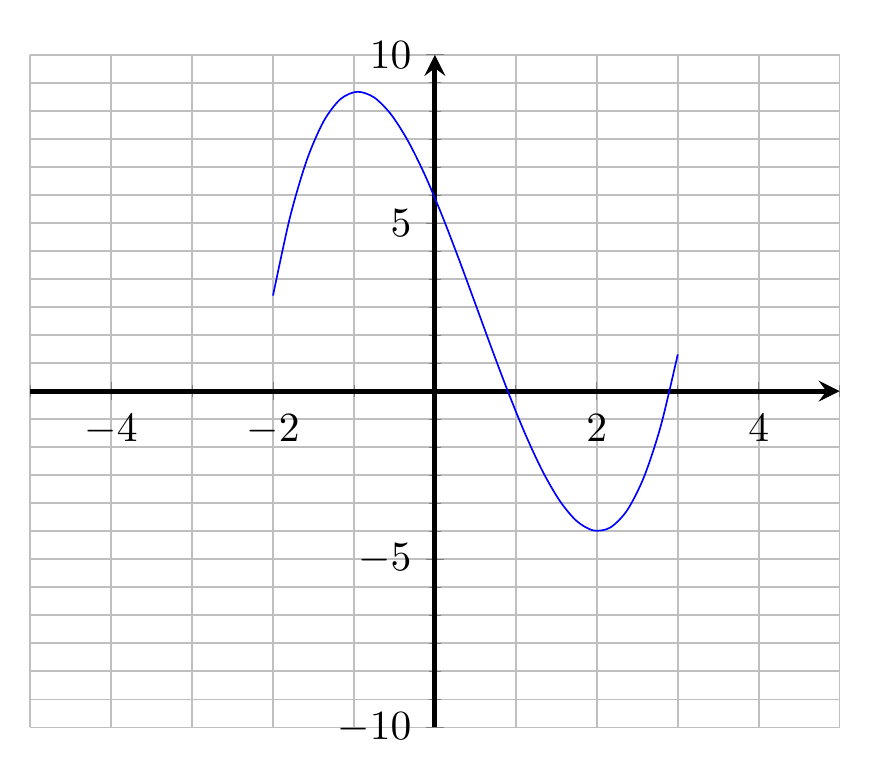
\begin{tikzpicture}[scale=1.5]
      \begin{axis}[
          xmin=-5,
          xmax=5,
          ymin=-10,
          ymax=10,
          axis lines=middle,
          grid=both,
          minor x tick num=1,
          minor y tick num=5,
          axis line style={very thick},
          clip=false
        ]
        \addplot [domain=-2:3,blue,smooth] {(x-1+0.1)*(x+2+0.2)*(x-3+0.1)};
      \end{axis}
  \end{tikzpicture}

  \vspace{0.25in}

  \begin{enumerate}
  \item Find the interval(s) where \(f\) is increasing and the interval(s) where \(f\) is decreasing.  Justify
    your answer.

    \newpage
    
  \item Find the \(x\) value of the relative/local maximum(s) of \(f\).  Justify your answer.

    \vspace{2in}

    
  \item Find the interval(s) of concavity of \(f\).  Justify your answer.

    \vspace{2in}
    
  \item Find the \(x\) value of the point(s) of inflection of \(f\).  Justify your answer.
  \end{enumerate}
\end{enumerate}

\end{document}
